\section{Model Equations}
\Figref{diagramQuad} shows a representation of the quadcopter where two reference systems, inertial and body, can be seen, as well as the conventions for angles of rotation and forces. \Figref{diagramTorque} shows the body from above and includes the chosen convention for the torques produced by the propellers.
 
\begin{minipage}{\linewidth}
	\begin{minipage}{0.45\linewidth}
		\begin{figure}[H]
			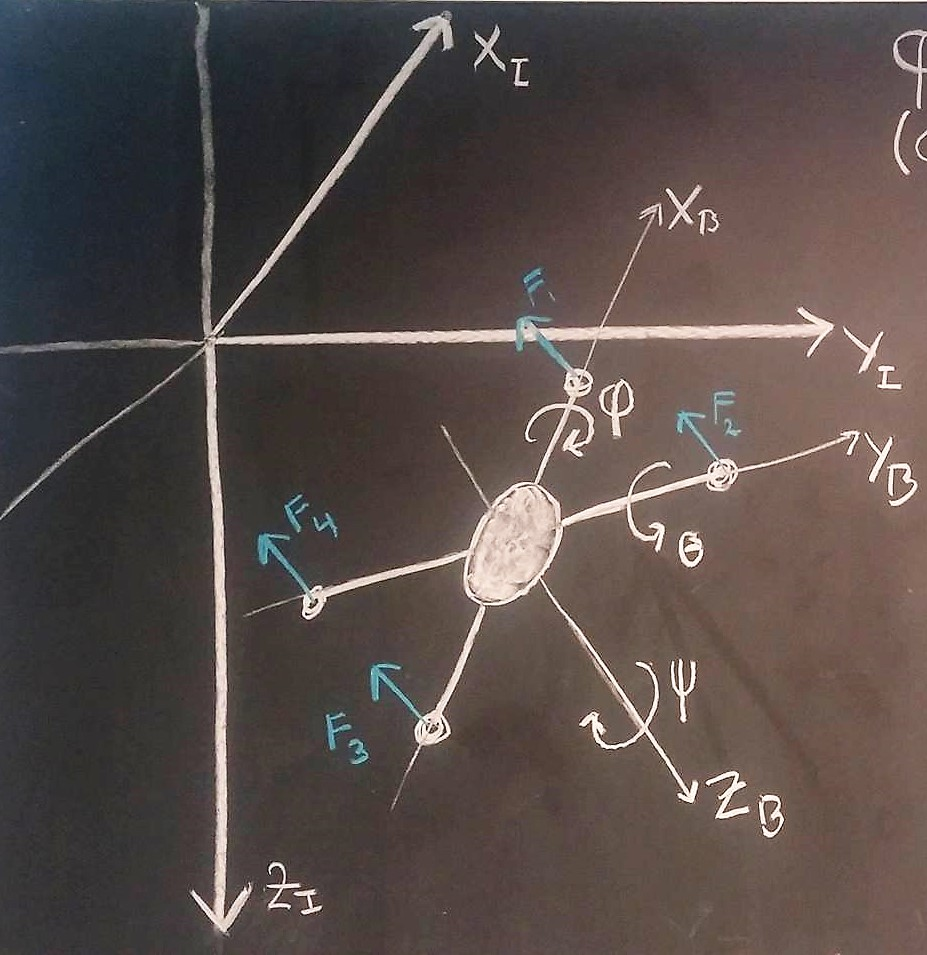
\includegraphics[scale=.27]{figures/drone_diagram}
			\centering
			\captionsetup{justification=centering}
			\captionof{figure}{Diagram of the quadcopter which includes inertial and body reference systems, as well as the references for the angles (roll, pitch and yaw) and the thrust forces produced by the propeller. }
			\label{diagramQuad}
		\end{figure}
	\end{minipage}
	\hspace{0.03\linewidth}
	\begin{minipage}{0.45\linewidth}
		\begin{figure}[H] \vspace{16mm}
			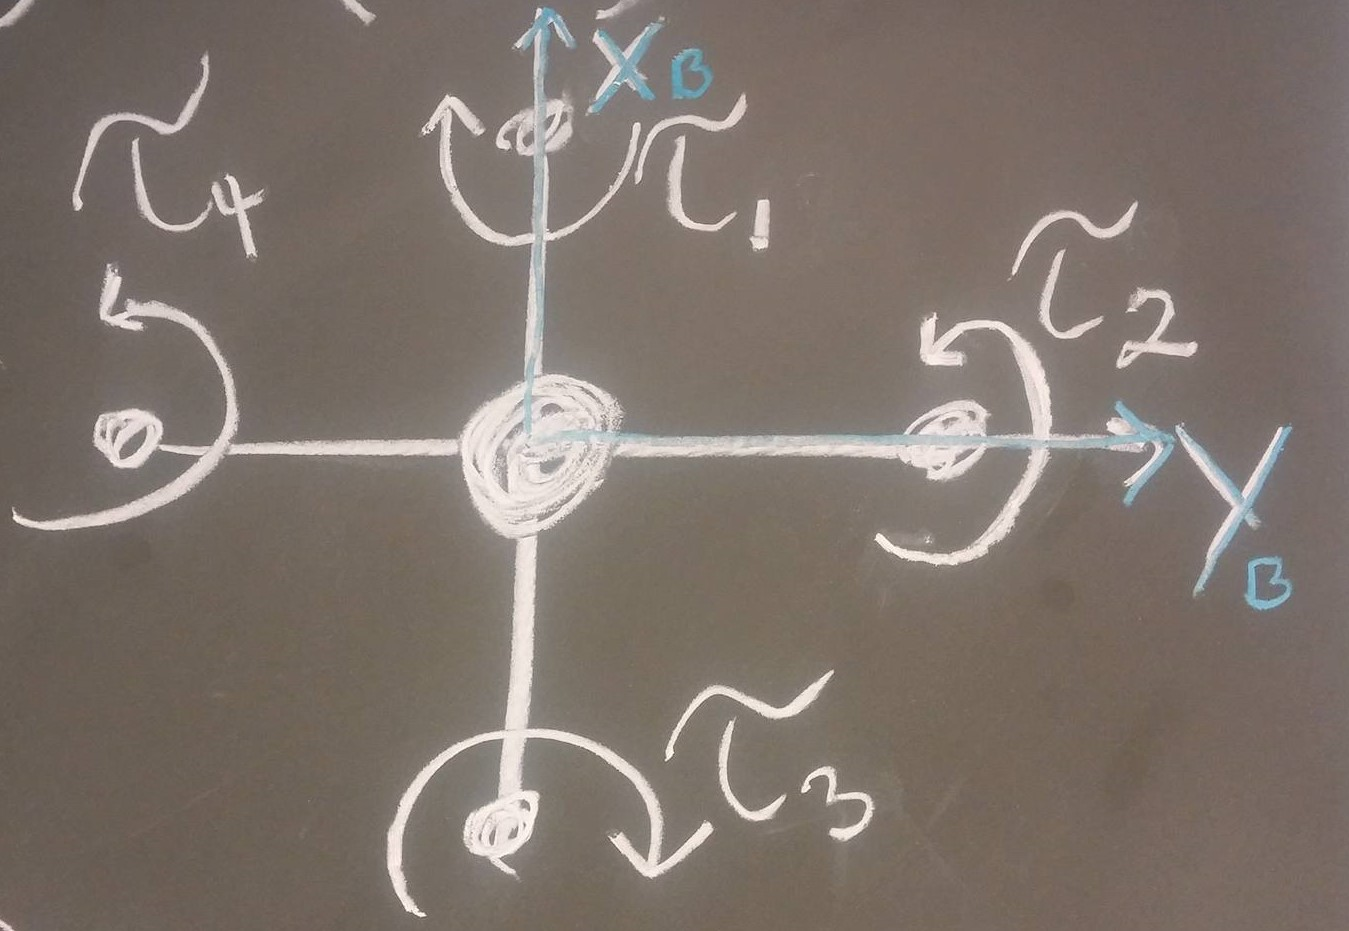
\includegraphics[scale=.18]{figures/torques_diagram}
			\centering
			\captionsetup{justification=centering}
			\captionof{figure}{Diagram of the quadcopter from above, with the references for the torques produced by the drag force at the propeller.}
			\label{diagramTorque}
		\end{figure}
	\end{minipage}
\end{minipage}
%
%\si{\phi} roll (around x-axis)\\ \\ 
%\si{\theta} pitch (around y-axis)\\ \\
%\si{\psi} yaw (around z-axis)\\
%

From the diagrams above, the equations of angular motion along the three body axes can be derived.
%
\begin{flalign}
\eq{ J_x\ddot{\phi} }{(F_4-F_2)L} &\\
\eq{J_y \ddot{\theta}}{(F_1-F_3)L} &\\
\eq{J_z\ddot{\psi}}{\tau_1-\tau_2+\tau_3-\tau_4}
\label{eq:AngleEq}
\end{flalign}

Where \si{\ddot{\phi}}, \si{\ddot{\theta}}, and \si{\ddot{\psi}} are the angular accelerations of the quadcopter in the roll, pitch and yaw angles; \si{J_x}, \si{J_y} and \si{J_z} represent the moment of inertia around each of the quadcopter axes, F represents the thrust force generated by each of the motors, L is the arm length of the quadcopter and \si{\tau} represents the torque generated by the drag force in each propeller.

As it can be seen in the \eqref{eq:AngleEq}, the roll and pitch angular accelerations depend on the thrust forces exerted by the propellers placed in the y and x axes of the quadcopter, respectively. The yaw angle changes only due to the torques created by the drag force in the propeller.

The linear acceleration components along the body coordinate frame directions evolve according to the equations below. They come from applying Newton's second law. As the gravity needs to be transformed from the inertial frame to the body frame, it has been multiplied by the rotation matrix (\eqref{rotMatrix}) that depends on the angles roll, pitch and yaw.
%
\begin{flalign}
\eq{F_g(\cos(\phi) \sin(\theta) \cos(\psi) + \sin(\phi) \sin (\psi))}{m\cdot\ddot{x}_B} &\\
\eq{F_g(\cos(\phi) \sin(\theta) \sin(\psi) - \sin(\phi) \cos(\psi))}{m\cdot\ddot{y}_B}&\\
\eq{-F_1-F_2-F_3-F_4+F_g\cdot \cos(\phi)\cos(\theta)}{m\cdot\ddot{z}_B} 
\label{eq:AccelerationEq}
\end{flalign}

Where \si{F_g} represents the gravitational force and \si{\ddot{x}_B}, \si{\ddot{y}_B}, and \si{\ddot{z}_B} represent the accelerations along the body axes of the quadcopter.

The trasformation of the gravity force is explained by three consecutive rotations (roll, pitch and yaw) combined in one rotation matrix \si{R_{\phi, \theta, \psi}}.

\begin{minipage}{0.3\linewidth}
\begin{flalign}
	\si{R_\phi} &=
	\begin{bmatrix}
		\ \si{1}                & \si{0}                & \si{0} \ \ \ \\ 
		\ \si{0}  				& \si{c(\phi)} 		& \si{-s(\phi)}                 \ \ \ \\ 
		\ \si{0}                & \si{s(\phi)}       & \si{c(\phi)}                  \ \ \  
	\end{bmatrix}  \nonumber 
\end{flalign}
\end{minipage}\hfill
%
\begin{minipage}{0.3\linewidth}
\begin{flalign}
	\si{R_\theta} &=
	\begin{bmatrix}
		\ \si{c(\theta)}      & \si{0}       & \si{s(\theta)} \ \ \ \\ 
		\ \si{0}  				& \si{1} 	   & \si{0}                 \ \ \ \\ 
		\ \si{-s(\theta)}     & \si{0}       & \si{c(\theta)}                  \ \ \  
	\end{bmatrix}   \nonumber 
\end{flalign}
\end{minipage}\hfill
%
\begin{minipage}{0.3\linewidth}
\begin{flalign}
	\si{R_\phi} &=
	\begin{bmatrix}
		\ \si{c(\psi)}                & \si{-s(\psi)}                & \si{0} \ \ \ \\ 
		\ \si{s(\psi)}  				& \si{c(\psi)} 		& \si{0}                 \ \ \ \\ 
		\ \si{0}                & \si{0}       & \si{1}                  \ \ \  
	\end{bmatrix} \nonumber 
\end{flalign}
\end{minipage}\hfill

\begin{flalign}
	\si{R_{\phi, \theta, \psi}} &=
	\begin{bmatrix}
		\ \si{c(\theta) \cdot c(\psi)}                & \si{-c(\theta) \cdot s(\psi)}  & \si{s(\theta)} \ \ \ \\ 
		\ \si{s(\phi) \cdot s(\theta) \cdot s(\psi) + c(\phi) \cdot s(\psi)}  	  & \si{-s(\phi) \cdot s(\theta) \cdot s(\psi) + c(\phi) \cdot c(\psi)} 		& \si{-s(\phi) \cdot c(\theta)}                 \ \ \ \\ 
		\ \si{-c(\phi) \cdot s(\theta) \cdot c(\psi) + s(\phi) \cdot s(\psi)}  	  & \si{c(\phi) \cdot s(\theta) \cdot s(\psi) + s(\phi) \cdot c(\psi)} 		& \si{c(\phi) \cdot c(\theta)}                 \ \ \ 
	\end{bmatrix} 	\label{rotMatrix}
\end{flalign}






